% file: chap6.tex

\chapter{深度学习}
\label{ch:Deeplearning}

在\hyperref[ch:WhyHardToTrain]{上一章},我们学习了深度神经网络通常比浅层神经网络
更加难以训练。我们有理由相信,若是可以训练深度网络,则能够获得比浅层网络更加强大
的能力,但是现实很残酷。从上一章我们可以看到很多不利的消息,但是这些困难不能阻止
我们使用深度神经网络。本章,我们将给出可以用来训练深度神经网络的技术,并在实战中
应用它们。同样我们也会从更加广阔的视角来看神经网络,简要地回顾近期有关深度神经网
络在图像识别、语音识别和其他应用中的研究进展。然后,还会给出一些关于未来神经网络
又或人工智能的简短的推测性的看法。

这一章比较长。为了更好地让你们学习,我们先粗看一下整体安排。本章的小结之间关联并
不太紧密,所以如果读者熟悉基本的神经网络的知识,那么可以任意跳到自己最感兴趣的部
分。

\hyperref[sec:convolutional_networks]{本章主要的部分}是对最为流行神经网络之一的深
度卷积网络的介绍。我们将细致地分析一个使用卷积网络来解决 MNIST 数据集的手写数字识
别的例子(包含了代码和讲解):
\begin{center}
  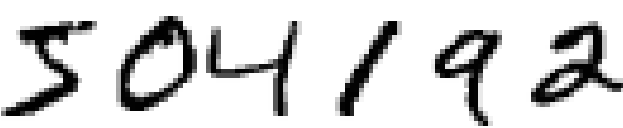
\includegraphics[width=64pt]{digits}
\end{center}

我们将从浅层的神经网络开始来解决上面的问题。通过多次的迭代,我们会构建越来越强大
的网络。在这个过程中,也将要探究若干强大技术:卷积、pooling、使用GPU来更好地训练、
训练数据的算法性扩展(避免过匹配)、dropout 技术的使用(同样为了防止过匹配现象)、
网络的 ensemble 使用 和 其他技术。最终的结果能够接近人类的表现。
在 10,000 幅 MNIST 测试图像上 —— 模型从未在训练中接触的图像 —— 该系统最终能够将其
中 9,967 幅正确分类。这儿我们看看错分的 33 幅图像。注意正确分类是右上的标记;系统
产生的分类在右下:
\begin{center}
  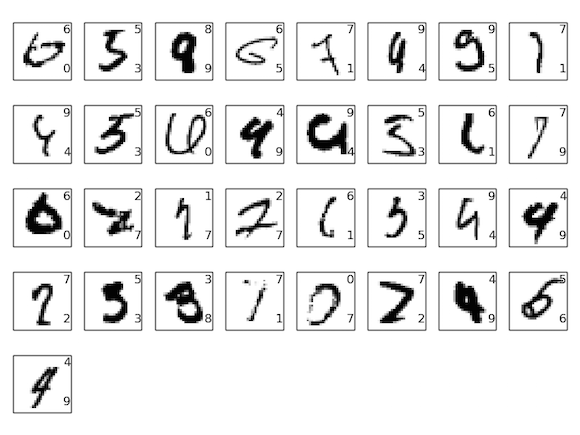
\includegraphics[width=.75\textwidth]{ensemble_errors}
\end{center}

可以发现,这里面的图像使对于人类来说都是非常困难区分的。例如,在第一行的第三幅图。
我看的话,看起来更像是 “9” 而非 “8”,而 “8” 却是给出的真实的结果。我们的网
络同样能够确定这个是 “9”。这种类型的“错误”最起码是容易理解的,可能甚至值得我
们赞许。最后用对最近使用深度(卷积)神经网络在图像识别上的研究进展作为关于图像识
别的讨论的总结。

本章剩下的部分,我们将会从一个更加宽泛和宏观的角度来讨论深度学习。概述一些神经网
络的其他模型,例如 RNN 和 LSTM 网络,以及这些网络如何在语音识别、自然语言处理和其
他领域中应用的。最后会试着推测一下,神经网络和深度学习未来发展的方向,会
从 intention-driven user interfaces 谈谈深度学习在人工智能的角色。这章内容建立在
本书前面章节的基础之上,使用了前面介绍的诸如 BP、规范化、softmax 函数,等等。然而,
要想阅读这一章,倒是不需要太过细致地掌握前面章节中内容的所有的细节。当然读完第一
章关于神经网络的基础是非常有帮助的。本章提到第二章到第五章的概念时,也会在文中给
出链接供读者去查看这些必需的概念。

需要注意的一点是,本章所没有包含的那一部分。这一章并不是关于最新和最强大的神经网
络库。我们也不是想训练数十层的神经网络来处理最前沿的问题。而是希望能够让读者理解
深度神经网络背后核心的原理,并将这些原理用在一个 MNIST 问题的解决中,方便我们的理
解。换句话说,本章目标不是将最前沿的神经网络展示给你看。包括前面的章节,我们都是
聚焦在基础上,这样读者就能够做好充分的准备来掌握众多的不断涌现的深度学习领域最新
工作。本章仍然在Beta版。期望读者指出笔误,bug,小错和主要的误解。如果你发现了可疑
的地方,请直接联系 mn@michaelnielsen.org。

\section{介绍卷积网络}
\label{sec:convolutional_networks}

在前面的章节中,我们教会了神经网络能够较好地识别手写数字:
\begin{center}
  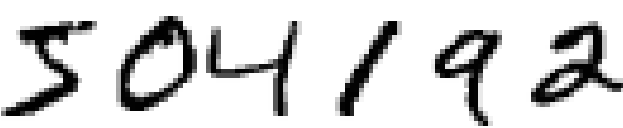
\includegraphics[width=64pt]{digits}
\end{center}

我们使用了全连接的邻接关系的网络来完成这个工作。即,网络中的神经元与相邻的层上的
每个神经元均连接:
\begin{center}
  \includegraphics{tikz41}
\end{center}

特别地,对输入图像中的每个像素点,我们将其光强度作为对应输入层神经元的值。对
于 $28 \times 28$ 像素的图像,这意味着我们的网络有
$784$($= 28 \times 28$)个输入神经元。我们然后训练网络的权重和偏置,使得网络输出
能够 —— 如我们希望地 —— 正确地辨认输入图像:'0', '1', '2', ..., '8', or '9'。

我们之前地网络工作得相当好:我们已经\hyperref[98percent]{得到了超过 98\% 的分类
  准确率},使用来自 \hyperref[sec:learning_with_gradient_descent]{MNIST 手写数字
  数据集}的训练和测试数据。但是仔细推敲,使用全连接层的网络来分类图像是很奇怪的。
原因是这样的一个网络架构不考虑图像的空间结构。例如,它在完全相同的基础上去对待相
距很远和彼此接近的输入像素。这样的空间结构的概念必须从训练数据中推断。但是如果我
们使用一个设法利用空间结构的架构,而不是从一个\emph{白板状态}的网络架构开始,会
怎样?在这一节中,我会描述\emph{卷积神经网络}\index{卷积神经网络}\footnote{The
  origins of convolutional neural networks go back to the 1970s. But the seminal
  paper establishing the modern subject of convolutional networks was a 1998
  paper, "Gradient-based learning applied to document recognition", by Yann
  LeCun, Léon Bottou, Yoshua Bengio, and Patrick Haffner. LeCun has since made
  an interesting remark on the terminology for convolutional nets: "The
  [biological] neural inspiration in models like convolutional nets is very
  tenuous. That's why I call them 'convolutional nets' not 'convolutional neural
  nets', and why we call the nodes 'units' and not 'neurons' ". Despite this
  remark, convolutional nets use many of the same ideas as the neural networks
  we've studied up to now: ideas such as backpropagation, gradient descent,
  regularization, non-linear activation functions, and so on. And so we will
  follow common practice, and consider them a type of neural network. I will use
  the terms "convolutional neural network" and "convolutional net(work)"
  interchangeably. I will also use the terms "[artificial] neuron" and "unit"
  interchangeably.}。这些网络使用一个特别适用于分类图像的特殊架构。使用这个架构
使得卷积网络能跟快训练。相应的,这帮助我们训练深度的、多层的网络,它非常擅长于分
类图像。今天,深度卷积网络或者一些近似的变化形式,被用在大多数图像识别的神经网络
中。

卷积神经网络采用了三种基本概念:\emph{局部感受野(local receptive
    fields\index{local receptive fields})},\emph{共享权重(shared
    weights\index{shared weights})},和\emph{混合(pooling\index{pooling})}。
让我们逐个看下:\\

\textbf{局部感受野\index{局部感受野}:} 在之前看到的全连接层的网络中,输入被描绘
成纵向排列的神经元。但在一个卷积网络中,把输入看作是一个 $28 \times 28$ 的方形排
列的神经元更有帮助,其值对应于我们用作输入的 $28 \times 28$ 的像素光强度:
\begin{center}
  \includegraphics{tikz42}
\end{center}

和通常一样,我们把输入像素连接到一个隐藏神经元层。但是我们不会把每个输入像素连接
到每个隐藏神经元。相反,我们只是把输入图像进行小的,局部区域的连接。

说的确切一点,第一个隐藏层中的每个神经元会连接到一个输入神经元的一个小区域,例如,
一个 $5 \times 5$ 的区域,对应于 $25$ 个输入像素。所以对于一个特定的隐藏神经元,
我们可能有看起来像这样的连接:
\begin{center}
  \includegraphics{tikz43}
\end{center}

这个输入图像的区域被称为隐藏神经元的\emph{局部感受野}。它是输入像素上的一个小窗口。
每个连接学习一个权重。而隐藏神经元同时也学习一个总的偏置。你可以把这个特定的隐藏
神经元看作是在学习分析它的局部感受野。

我们然后在整个输入图像上交叉移动局部感受野。对于每个局部感受野,在第一个隐藏层中
有一个不同的隐藏神经元。为了正确说明,让我们从左上角开始一个局部感受野:
\begin{center}
  \includegraphics{tikz44}
\end{center}

然后我们往右一个像素(即一个神经元)移动局部感受野,连接到第二个隐藏神经元:
\begin{center}
  \includegraphics{tikz45}
\end{center}

如此重复,构建起第一个隐藏层。注意如果我们有一个 $28 \times 28$ 的输入图像,$5
\times 5$ 的局部感受野,那么隐藏层中就会有 $24 \times 24$ 个神经元。这是因为在抵
达右边(或者底部)的输入图像之前,我们只能把局部感受野横向移动 $23$ 个神经元(或
  者往下 $23$ 个神经元)。

我显示的局部感受野每次移动一个像素。实际上,有时候会使用不同的\emph{跨距}。例如,
我可以往右(或下)移动 $2$ 个像素的局部感受野,这种情况下我们使用了 $2$ 个跨距。
在这章里我们大部分时候会固定使用 $1$ 的跨距,但是值得知道人们有时用不同的跨距试
验\footnote{As was done in earlier chapters, if we're interested in trying
  different stride lengths then we can use validation data to pick out the
  stride length which gives the best performance. For more details, see the
  \hyperref[sec:how_to_choose_a_neural_network's_hyper-parameters]{earlier
    discussion} of how to choose hyper-parameters in a neural network. The same
  approach may also be used to choose the size of the local receptive field -
  there is, of course, nothing special about using a $5 \times 5$ local
  receptive field. In general, larger local receptive fields tend to be helpful
  when the input images are significantly larger than the $28 \times 28$ pixel
  MNIST images.}。\\

\textbf{共享权重\index{共享权重}和偏置:} 我已经说过每个隐藏神经元具有一个偏置和
连接到它的局部感受野的 $5 \times 5$ 权重。我没有提及的是我们打算对 $24 \times
24$ 隐藏神经元中的每一个使用\emph{相同的}权重和偏置。换句话说,对第 $j, k$ 个隐
藏神经元,输出为:
\begin{equation}
  \sigma\left(b + \sum_{l=0}^4 \sum_{m=0}^4  w_{l,m} a_{j+l, k+m} \right)
  \label{eq:125}\tag{125}
\end{equation}

这里 $\sigma$ 是神经元的激活函数 —— 可以是我们在前面章里使用过的
\hyperref[sec:sigmoid_neurons]{S型函数}。$b$ 是偏置的共享值。$w_{l,m}$ 是一个共
享权重的 $5 \times 5$ 数组。最后,我们使用 $a_{x, y}$ 来表示位置为 $x, y$ 的输入
激活值。

这意味着第一个隐藏层的所有神经元检测完全相同的特征\footnote{我还没有精确定义特征
  的概念。非正式地,把一个隐藏神经元检测的特征看作一种引起神经元激活的输入模式:
  例如,它可能是图像的一条边,或者一些其它的形状。},只是在输入图像的不同位置。
要明白为什么是这个道理,把权重和偏置设想成隐藏神经元可以挑选的东西,例如,在一个
特定的局部感受野的垂直边缘。这种能力在图像的其它位置也很可能是有用的。因此,在图
像中应用相同的特征检测器是非常有用的。用稍微更抽象的术语,卷积网络能很好地适应图
像的平移不变性:例如稍稍移动一幅猫的图像,它仍然是一幅猫的图像\footnote{In fact,
  for the MNIST digit classification problem we've been studying, the images are
  centered and size-normalized. So MNIST has less translation invariance than
  images found "in the wild", so to speak. Still, features like edges and
  corners are likely to be useful across much of the input space.}。

因为这个原因,我们有时候把从输入层到隐藏层的映射称为一个\emph{特征映射}。我们把
定义特征映射的权重称为\emph{共享权重}。我们把以这种方式定义特征映射的偏置称为%
\emph{共享偏置}。共享权重和偏置经常被称为一个\emph{卷积核}或者\emph{滤波器}。在文献
中,人们有时以稍微不同的方式使用这些术语,对此我不打算去严格区分;稍后我们会看一
些具体的例子。

目前我描述的网络结构只能检测一种局部特征的类型。为了完成图像识别我们需要超过一个
的特征映射。所以一个完整的卷积层由几个不同的特征映射组成:
\begin{center}
  \includegraphics{tikz46}
\end{center}

在这个例子中,有 3 个特征映射。每个特征映射定义为一个 $5 \times 5$ 共享权重和单个
共享偏置的集合。其结果是网络能够检测 3 种不同的特征,每个特征都在整个图像中可检
测。

为了让上面的图示简单些,我仅仅展示了 $3$ 个特征映射。然而,在实践中卷积网络可能使
用很多(也许多得多)的特征映射。一种早期的识别 MNIST 数字的卷积网络,LeNet-5,使
用 $6$ 个特征映射,每个关联到一个 $5 \times 5$ 的局部感受野。所以上面的插图例子实
际和 LeNet-5 很接近。而在我们在本章后面要开发的例子里,我们将使用具有 20 和40 个
特征映射的卷积层。让我们快速看下已经学到的一些特征\footnote{The feature maps
  illustrated come from the final convolutional network we train, see here.}:
\begin{center}
  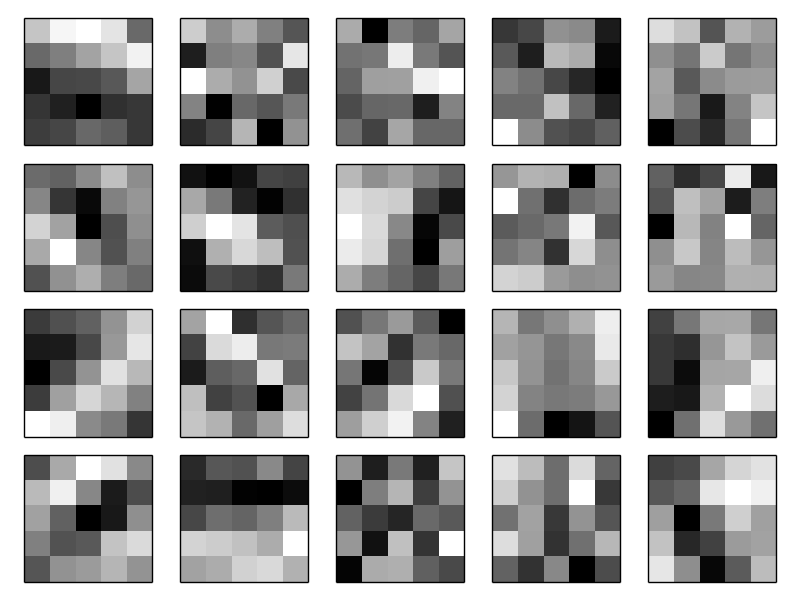
\includegraphics[width=.65\textwidth]{net_full_layer_0}
\end{center}

这 20 幅图像对应于 20 个不同的特征映射(或滤波器、核)。每个映射有一幅 $5 \times
5$ 块的图像表示,对应于局部感受野中的 $5 \times 5$ 权重。白色块意味着一个小(典型
的,更小的负数)权重,所以这样的特征映射对相应的输入像素有更小的响应。更暗的块意
味着一个更大的权重,所以这样的特征映射对相应的输入像素有更大的响应。非常粗略地讲,
上面的图像显示了卷基层作出响应的特征类型。

所以我们能从这些特征映射中得到什么结论?很明显这里有超出了我们期望的空间结构:这
些特征许多有清晰的亮和暗的子区域。这表示我们的网络实际上正在学习和空间结构相关的
东西。然而,除了那个,看清这些特征检测器在学什么是很困难的。当然,我们并不是在学
习(例如)\href{http://en.wikipedia.org/wiki/Gabor_filter}{Gabor 滤波器},它已经
被用在很多传统的图像识别方法中。实际上,现在有许多关于通过卷积网络来更好理解特征
的工作成果。如果你感兴趣,我建议从 Matthew Zeiler 和 Rob Fergus 的(2013)论
文 \href{http://arxiv.org/abs/1311.2901}{Visualizing and Understanding
  Convolutional Networks} 开始。

共享权重和偏置的一个很大的优点是,它大大减少了参与的卷积网络的参数。对于每个特征
映射我们需要 $25 = 5 \times 5$ 个共享权重,加上一个共享偏置。所以每个特征映射需
要 $26$ 个参数。如果我们有 $20$ 个特征映射,那么总共有 $20 \times 26 = 520$ 个参
数来定义卷积层。作为对比,假设我们有一个全连接的第一层,具有 $784 = 28 \times
28$ 个输入神经元,和一个相对适中的 $30$ 个隐藏神经元,正如我们在本书之前的很多例
子中使用的。总共有 $784 \times 30$ 个权重,加上额外的 $30$ 个偏置,共
有 $23,550$个参数。换句话说,这个全连接的层有多达 $40$ 倍于卷基层的参数。

当然,我们不能真正做一个参数数量之间的直接比较,因为这两个模型的本质是不同的径。
但是,直观地,使用卷积层的平移不变性似乎很可能减少全连接模型中达到同样性能的参数
数量。反过来,这将导致更快的卷积模型的训练,并最终,将有助于我们使用卷基层建立度
深网络。

顺便提一下,\emph{卷积}(\textit{convolutional})这一名称源自方
程~\eqref{eq:125}中的操作符有时被称为一个\emph{卷积}(\textit{convolution})。稍
微更精确些,人们有时把这个方程写成 $a^1 = \sigma(b + w * a^0)$,其中 $a^1$ 表示出
自一个特征映射的输出激活值集合,$a^0$ 是输入激活值的集合,而 $*$ 被称为一个卷积操
作。我们不打
算深入使用卷积数学,所以你不用对此太担心。但是至少值得知道这个名称从何而来。\\

\textbf{混合层:} 除了刚刚描述的卷积层,卷积神经网络也包含\emph{混合
  层}(\textit{pooling layers})。混合层通常紧接着在卷积层之后使用。它要做的
简化从卷积层输出的信息。

详细地说,一个混合层取得从卷积层输出的每一个特征映射\footnote{The
  nomenclature is being used loosely here. In particular, I'm using "feature
  map" to mean not the function computed by the convolutional layer, but rather
  the activation of the hidden neurons output from the layer. This kind of mild
  abuse of nomenclature is pretty common in the research literature.}并且从它们准
备一个凝缩的特征映射。例如,混合层的每个单元可能概括了前一层的一个(比如)$2
\times 2$ 的区域。作为一个具体的例子,一个常见的混合的程序被称为\emph{最大值混
  合}(\textit{max-pooling})。在最大值混合中,一个混合单元简单地输出
其 $2 \times 2$ 输入区域的最大激活值,正如下图说明的:
\begin{center}
  \includegraphics{tikz47}
\end{center}
注意既然从卷积层有 $24 \times 24$ 个神经元输出,混合后我们得到 $12 \times
12$ 个神经元。

正如上面提到的,卷积层通常包含超过一个特征映射。我们将最大值混合分别应用于每一
个特征映射。所以如果有三个特征映射,组合在一起的卷积层和最大值混合层看起来像这
样:
\begin{center}
  \includegraphics{tikz48}  
\end{center}

我们可以把最大值混合看作一种网络询问是否有一个给定的特征在一个图像区域中的哪个
地方被发现的方式。然后它扔掉确切的位置信息。直观上,一旦一个特征被发现,它的确切
位置并不如它相对于其它特征的大概位置重要。一个很大的好处是,这样可以有很多被更少
地混合的特征,所以这有助于减少在以后的层所需的参数的数目。

最大值混合并不是用于混合的仅有的技术。另一个常用的方法是\emph{L2 混合}(\textit{L2
    pooling})。这里我们取 $2 \times 2$ 区域中激活值的平方和的平方根,而不是最大
激活值。虽然细节不同,但其直观上和最大值混合是相似的:L2 混合是一种凝缩从卷积层输
出的信息的方式。在实践中,两种技术都被广泛应用。而且有时候人们使用其它混合操作的
类型。如果你正在尝试优化性能,你可以使用验证数据来比较混合的不同方法,并选择一个
工作得最好的。但我们不打算惦记这种细节上的优化。\\

\textbf{综合在一起:} 我们现在可以把这些思想都放在一起来构建一个完整的卷积神经网
络。它和我们刚看到的架构相似,但是有额外的一层 $10$ 个输出神经元,对应于 $10$ 个
可能的 MNIST 数字('0','1','2'等):
\begin{center}
  \includegraphics{tikz49}  
\end{center}

这个网络从 $28 \times 28$ 个输入神经元开始,这些神经元用于对 MNIST 图像的像素强度
进行编码。接着的是一个卷积层,使用一个 $5 \times 5$ 局部感受野和 $3$ 个特征映射。
其结果是一个 $3 \times 24 \times 24$ 隐藏特征神经元层。下一步是一个最大值混合层,
应用于$2 \times 2$ 区域,遍及 $3$ 个特征映射。结果是一个 $3 \times 12 \times 12$
隐藏特征神经元层。

网络中最后连接的层是一个全连接层。更确切地说,这一层将最大值混合层的\emph{每一个}神
经元连接到每一个输出神经元。这个全连接结构和我们之前章节中使用的相同。然而,注意
上面的图示,为了简化,我只使用了一个箭头,而不是显示所有的连接。当然,你可以很容
易想象到这些连接。

这个卷积架构和之前章节中使用的架构相当不同。但是总体的描述是相似的:一个由很多简
单的单元构成的网络,这些单元的行为由它们的权重和偏置确定。而总体的目标仍然是一样
的:用训练数据来训练网络的权重和偏置,使得网络可以胜任分类输入数字。

特别的,正如本书中前面那样,我们将用随即梯度下降和反向传播训练我们的网络。这大部
分按照前面章节中完全相同的方式来处理。然而,我们确实需要对反向传播程序做些修改。
原因是我们之前的\hyperref[ch:HowThebackpropagationalgorithmworks]{反向传播的推导}是
针对全连接层的网络。幸运的是,针对卷积和最大值混合层的推导是简单的。如果你想理解细
节,那么我请你完成下面的问题。注意这个问题会花费些时间来完成,除非你确实已经吸收
了\hyperref[ch:HowThebackpropagationalgorithmworks]{之前的反向传播的推导}(这种
  情况下是容易的)。

\subsection*{问题}

\begin{itemize}
\item \textbf{卷积网络中的反向传播}\quad 在一个具有全连接层的网络中,反向传播的核
  心方程是 \eqref{eq:bp1}--\eqref{eq:bp4}(\hyperref[backpropsummary]{链接})。假
  设我们有这样一个网络,它包含有一个卷积层,一个最大值混合层,和一个全连接的输出层,
  正如上面讨论的那样。反向传播的方程式要如何修改?
\end{itemize}

\section{卷积神经网络在实际中的应用}
\label{seq:convolutional_neural_networks_in_practice}

我们现在已经明白了卷积神经网络后面的核心思想。让我们通过实现一些卷积网络,并将它
们应用于 MNIST 数字分类问题,来看看它们如何在实践中工作。我们将使用的程序
是 \lstinline!network3.py!,它是前面章节开发
的 \lstinline!network.py! 和 \lstinline!network2.py! 的强化版本\footnote{Note
  also that network3.py incorporates ideas from the Theano library's
  documentation on convolutional neural nets (notably the implementation of
  LeNet-5), from Misha Denil's implementation of dropout, and from Chris Olah.}。
如果你想跟着学,代码可以
从
\href{https://github.com/mnielsen/neural-networks-and-deep-learning/blob/master/src/network3.py}{GitHub}
上下载。注意我们将在下一节中解决 \lstinline!network3.py! 需要的代码。在这一节中,
我们将把 \lstinline!network3.py! 作为库来构建卷积网络。

程序 \lstinline!network.py! 和 \lstinline!network2.py! 是用 Python 和矩阵
库 Numpy 实现的。这些程序从最初的原理工作,并致力于反向传播、随即梯度下降等细节。
但是现在我们已经理解了这些细节,对于 \lstinline!network3.py! 我们打算使用一个称
为 \href{http://deeplearning.net/software/theano/}{Theano} 的机器学习
库\footnote{See Theano: A CPU and GPU Math Expression Compiler in Python, by
  James Bergstra, Olivier Breuleux, Frederic Bastien, Pascal Lamblin, Ravzan
  Pascanu, Guillaume Desjardins, Joseph Turian, David Warde-Farley, and Yoshua
  Bengio (2010). Theano is also the basis for the popular Pylearn2 and Keras
  neural networks libraries. Other popular neural nets libraries at the time of
  this writing include Caffe and Torch.}。使用 Theano 使得实现针对卷积神经网络的
反向传播很容易,因为它自动计算涉及到的映射。Theano 也比我们前面代码更快(那些代码
是为了容易理解,不是为了运行速度),这使它可实际用于训练更复杂的网络。特别
地,Theano 的一个非常好的特性是它能够运行于 CPU 或者,如果可以,GPU 上。运行
于 GPU 上可以提供显著的增速,而且,有助于实际用于更复杂的网络。

如果你想要跟着学,你需要可运行在你的系统上的 Theano。按照项
目\href{http://deeplearning.net/software/theano/}{主页}上的说明来安装 Theano。接
下来的例子使用 Theano 0.6\footnote{As I release this chapter, the current
  version of Theano has changed to version 0.7. I've actually rerun the examples
  under Theano 0.7 and get extremely similar results to those reported in the
  text.} 运行过。有些在没有 GPU 支持的 Mac OS X Yosemite 运行过。有些在有 NVIDIA
GPU 支持的 Ubuntu 14.04 中运行过。有些实验在两个系统中都运行过。为了
让 \lstinline!networks3.py! 运行,你需要(适当地)把 \lstinline!networks3.py! 源
码中的 \lstinline!GPU! 标志设置为 \lstinline!True! 或者 \lstinline!False!。此外,
为了让 Theano 运行于 GPU 上,你可能会发
现\href{http://deeplearning.net/software/theano/tutorial/using_gpu.html}{这份指导
  说明}有帮助。互联网上也有教程,很容易用 Google 搜索到,同样能帮助你让 Theano 工
作。如果你手上的系统没有可用的 GPU,那么你可能想要看
下 \href{http://aws.amazon.com/ec2/instance-types/}{Amazon Web Services} EC2 G2
实例类型。注意即使有 GPU 支持,代码仍然需要一些时间执行。许多实验要花费从几分钟到
几个小时的时间来运行。在 CPU 上可能需要花费数天时间来运行最复杂的实验。正如前面章
节里说的,我建议让程序运行着,同时继续阅读,偶尔回来检查下代码的输出。如果你用的
是 CPU,你可能需要对更复杂的实验减少训练\epochs{}的数量,或者整个忽略它们。

为了取得一个基线,我们将从一个浅层架构开始,它仅仅使用一个隐藏层,包含 $100$ 个隐
藏神经元。我们会训练 $60$ \epochs{},使用\learningrate{}为:$\eta =
0.1$,\minibatch{} 大小为 $10$,没有规范化。这样运行\footnote{Code for the
  experiments in this section may be found in this script. Note that the code in
  the script simply duplicates and parallels the discussion in this section.}:
\begin{lstlisting}[language=Python]
>>> import network3
>>> from network3 import Network
>>> from network3 import ConvPoolLayer, FullyConnectedLayer, SoftmaxLayer
>>> training_data, validation_data, test_data = network3.load_data_shared()
>>> mini_batch_size = 10
>>> net = Network([
        FullyConnectedLayer(n_in=784, n_out=100),
        SoftmaxLayer(n_in=100, n_out=10)], mini_batch_size)
>>> net.SGD(training_data, 60, mini_batch_size, 0.1, 
            validation_data, test_data)
\end{lstlisting}

我获得的一个最好的分类准确率是 $97.80$\%。这是 \lstinline!test_data! 上的分类准确
率,在这个取值的训练\epoch{}的地方,我们在\lstinline!validation_data!上得到了最好
的分类准确率。使用验证数据来决定在何时对测试准确率估值有助于避免测试数据上的过度
拟合(见前面关于验证数据使用的\hyperref[validation_explanation]{讨论})。我们将在
下面遵循这个习惯。你的结构可能稍有不同,因为网络的权重和偏置是随机初始化
的\footnote{In fact, in this experiment I actually did three separate runs
  training a network with this architecture. I then reported the test accuracy
  which corresponded to the best validation accuracy from any of the three
  runs. Using multiple runs helps reduce variation in results, which is useful
  when comparing many architectures, as we are doing. I've followed this
  procedure below, except where noted. In practice, it made little difference to
  the results obtained.}。

这个 $97.80$\% 的准确率接近于\hyperref[chap3_98_04_percent]{第三章}中获得
的 $98.04$\% 的准确率,使用一个相似的网络架构和学习超参数。特别地,两个例子都使用
一个浅层网络,具有单个包含有 $100$ 个隐藏神经元的隐藏层。两者都训
练 $60$ 个\epochs{},\minibatch{}大小为 $10$,\learningrate{} 为 $\eta = 0.1$。

然而,在之前的网络中有两个不同的地方。首先,我
们\hyperref[sec:overfitting_and_regularization]{规范化}了之前的网络,来帮助降低过
度拟合带来的影响。规范化当前的网络确实可以提高准确率,但是得到的只是很小,所以我
们将推迟到后面再来惦记规范化。第二,虽然之前的网络中的最终层使用了S型激活值和交叉
熵代价函数,当前网络使用一个柔性最大值的最终层,以及对数似然代价函数。正如第三章
中\hyperref[subsec:softmax]{解释}的,这不是一个大的改变。我没有为了任何特别深刻的
原因来做出这样的改变 —— 主要是因为柔性最大值和对数似然代价在现代的图像分类网络中
很常见。

我们能用一个更深的网络架构来做得比这些结果更好吗?

让我们从在网络开始位置的右边插入一个卷积层开始。我们将使用 $5 \times 5$ 局部感受
野,跨距为 $1$,$20$ 个特征映射。我们也会插入一个最大值混合层,它用一个 $2
\times 2$ 的混合窗口来合并特征。所以总体的网络架构看起来很像上一节讨论的架构,但
是有一个额外的全连接层:
\begin{center}
  \includegraphics{simple_conv}  
\end{center}

在这个架构中,我们可以把卷积和混合层看作是在学习输入训练图像中的局部感受野,而后
面的全连接层则在一个更抽象的层次学习,从整个图像整合全局信息。这是一种常见的卷积
神经网络模式。

让我们训练这样的一个网络,看看它表现怎样\footnote{I've continued to use a
  mini-batch size of $10$ here. In fact, as we
  \hyperref[mini_batch_size]{discussed earlier} it may be possible to speed up
  training using larger mini-batches. I've continued to use the same mini-batch
  size mostly for consistency with the experiments in earlier chapters.}:

\begin{lstlisting}[language=Python]
>>> net = Network([
        ConvPoolLayer(image_shape=(mini_batch_size, 1, 28, 28), 
                      filter_shape=(20, 1, 5, 5), 
                      poolsize=(2, 2)),
        FullyConnectedLayer(n_in=20*12*12, n_out=100),
        SoftmaxLayer(n_in=100, n_out=10)], mini_batch_size)
>>> net.SGD(training_data, 60, mini_batch_size, 0.1, 
            validation_data, test_data)
\end{lstlisting}

我们得到了 $98.78$\% 的准确率,这是相当大的改善,超过了我们以前结构的任何一个。事
实上,我们已经减少了超过三分之一的错误率,这是一个很大的进步。

在指定网络结构时,我把卷积和混合层作为一个单一层对待。不管他们是被视为分开的
层还是作为一个单一的层在一定程度上是一个个人喜好的问题。\lstinline!network3.py!
视他们为单个层,因为它使得 \lstinline!network3.py! 的代码更紧凑。然而,如果需要的
话,很容易修改 \lstinline!network3.py! 使得这些层可以单独指定。

\subsection*{练习}

\begin{itemize}
\item 如果你删除了全连接层,只使用卷积--混合层和柔性最大值层,你得到了什么样的分类准确率?
全连接层的加入有帮助吗?
\end{itemize}

我们能改进 $98.78$\% 的分类准确率吗?

让我们试着插入第二个卷积--混合层。把它插在已有的卷积--混合层和全连接隐藏
层之间。我们再次使用一个 $5 \times 5$ 局部感受野,混合 $2 \times 2$ 的区域。
让我们看看用前面相似的超参数训练会发生什么:
\begin{lstlisting}[language=Python]
>>> net = Network([
        ConvPoolLayer(image_shape=(mini_batch_size, 1, 28, 28), 
                      filter_shape=(20, 1, 5, 5), 
                      poolsize=(2, 2)),
        ConvPoolLayer(image_shape=(mini_batch_size, 20, 12, 12), 
                      filter_shape=(40, 20, 5, 5), 
                      poolsize=(2, 2)),
        FullyConnectedLayer(n_in=40*4*4, n_out=100),
        SoftmaxLayer(n_in=100, n_out=10)], mini_batch_size)
>>> net.SGD(training_data, 60, mini_batch_size, 0.1, 
            validation_data, test_data)        
\end{lstlisting}

再一次,我们得到了改善:现在我们达到了 $99.06$\% 的分类准确率。

在这里有两个很自然想到的问题。第一个问题是:应用第二个卷积--混合层意味着什么?
实际上,你可以认为第二个卷积--混合层输入 $12 \times 12$ 幅“图像”,其“像素”
代表原始输入图像中特定的局部特征的存在(或不存在)。所以你可以认为这一层输入原始
输入图像的一个版本。这个版本是经过抽象和凝缩过的,但是仍然有大量的空间结构,所以
使用第二个卷积--混合层是有意义的。

这是一个令然满意的观点,但是引出了第二个问题。从前面层的输出涉及 $20$ 个独立的特
征映射,所以对第二个卷积--混合层有 $20 \times 20 \times 12$ 个输入。就好像我们
有 $20$ 幅单独的图像输入给卷积--混合层,而不是第一个卷积--混合层情况下的单幅图像。
第二个卷积--混合层里的神经元应该如何响应这些多重的输入图像呢?实际上,我们将允许
这一层中的每个神经元从它的局部感受野中的\emph{所有} $20 \times 5 \times 5$ 输入神
经元学习。更非正式的:第二个卷积--混合层中的特征检测器可访问\emph{所有}前面层的特
征,但仅在其特定的局部感受野中\footnote{This issue would have arisen in the
  first layer if the input images were in color. In that case we'd have 3 input
  features for each pixel, corresponding to red, green and blue channels in the
  input image. So we'd allow the feature detectors to have access to all color
  information, but only within a given local receptive field.}。

\subsection*{问题}

\begin{itemize}
\item \textbf{使用 tanh 激活函数}\quad 在本书前面我已经几次提起
  过\hyperref[subsec:other_models_of_artificial_neuron]{tanh 函数}可以是一个
  比 S型函数更好的激活函数。我们还没有实际采用过这些建议,因为我们已经用 S 型取得
  了大量进展。但现在让我们试试一些用 tanh 作为我们激活函数的实验。试着训练卷积和
  全连接层中具有 tanh 激活值的网络\footnote{Note that you can pass
    \lstinline!activation_fn=tanh! as a parameter to the
    \lstinline!ConvPoolLayer! and \lstinline!FullyConnectedLayer! classes.}。开始
  时使用 S 型网络中使用的相同的超参数,但是训练 $20$ 个\epochs{},而不是 $60$ 个。
  你的网络表现得怎么样?如果你继续训练到 $60$ 个\epochs{}会怎样?试着
  将tanh 和 S型网络的每个\epoch{}的验证准确率都绘制出来,都绘制
  到 $60$ 个\epochs{}。如果你的结果和我的相似,你会发现 tanh 网络训练得稍微快些,
  但是最终的准确率非常相似。你能否解释为什么 tanh 网络可以训练得更快?你能否用 S
  型取得一个相似的训练速度,也许通过改变\learningrate{},或者做些调
  整\footnote{You may perhaps find inspiration in recalling that
    $\sigma(z) = (1+\tanh(z/2))/2$.}?试着用五六个迭代学习超参数和网络架构,寻
  找 tanh 优于 S 型的方面。\emph{注意:这是一个开放式问题。就我个人而言,我并没有
    找到太多切换为 tanh 的优势,虽然我没全面地做过实验,也许你会找到一个方法。无
    论如何,我们马上会发现切换到修正线性激活函数的一个优势,所以我们不会去深入使
    用 tanh 函数。}。
\end{itemize}

\textbf{使用修正线性单元:} 到现在我们开发的网络实际上是一个在开创性的 1998 论文
中使用的网络的变化形式。

\begin{lstlisting}[language=Python]
>>> from network3 import ReLU
>>> net = Network([
        ConvPoolLayer(image_shape=(mini_batch_size, 1, 28, 28), 
                      filter_shape=(20, 1, 5, 5), 
                      poolsize=(2, 2), 
                      activation_fn=ReLU),
        ConvPoolLayer(image_shape=(mini_batch_size, 20, 12, 12), 
                      filter_shape=(40, 20, 5, 5), 
                      poolsize=(2, 2), 
                      activation_fn=ReLU),
        FullyConnectedLayer(n_in=40*4*4, n_out=100, activation_fn=ReLU),
        SoftmaxLayer(n_in=100, n_out=10)], mini_batch_size)
>>> net.SGD(training_data, 60, mini_batch_size, 0.03, 
            validation_data, test_data, lmbda=0.1)
\end{lstlisting}

\textbf{扩展训练数据:}

\subsection*{问题}

\textbf{插入一个额外的全连接层:}

\textbf{使用一个整体网络:}

\begin{center}
  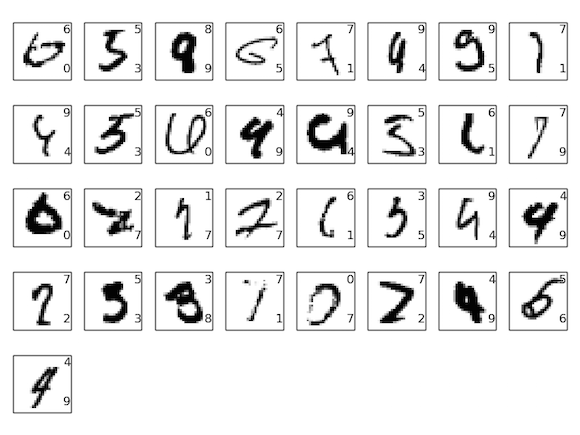
\includegraphics[width=.75\textwidth]{ensemble_errors}
\end{center}

\textbf{为什么我们只对全连接层应用弃权:}

\textbf{进一步:}

\textbf{为什么我们能够训练?}

\textbf{这些网络有多深?}

\textbf{A word on procedure:}

\section{卷积网络的代码}
\label{sec:the_code_for_our_convolutional_networks}

\begin{lstlisting}[language=Python]
class FullyConnectedLayer(object):

    def __init__(self, n_in, n_out, activation_fn=sigmoid, p_dropout=0.0):
        self.n_in = n_in
        self.n_out = n_out
        self.activation_fn = activation_fn
        self.p_dropout = p_dropout
        # Initialize weights and biases
        self.w = theano.shared(
            np.asarray(
                np.random.normal(
                    loc=0.0, scale=np.sqrt(1.0/n_out), size=(n_in, n_out)),
                dtype=theano.config.floatX),
            name='w', borrow=True)
        self.b = theano.shared(
            np.asarray(np.random.normal(loc=0.0, scale=1.0, size=(n_out,)),
                       dtype=theano.config.floatX),
            name='b', borrow=True)
        self.params = [self.w, self.b]

    def set_inpt(self, inpt, inpt_dropout, mini_batch_size):
        self.inpt = inpt.reshape((mini_batch_size, self.n_in))
        self.output = self.activation_fn(
            (1-self.p_dropout)*T.dot(self.inpt, self.w) + self.b)
        self.y_out = T.argmax(self.output, axis=1)
        self.inpt_dropout = dropout_layer(
            inpt_dropout.reshape((mini_batch_size, self.n_in)), self.p_dropout)
        self.output_dropout = self.activation_fn(
            T.dot(self.inpt_dropout, self.w) + self.b)

    def accuracy(self, y):
        "Return the accuracy for the mini-batch."
        return T.mean(T.eq(y, self.y_out))
\end{lstlisting}

\begin{lstlisting}[language=Python]
class Network(object):
    
    def __init__(self, layers, mini_batch_size):
        """Takes a list of `layers`, describing the network architecture, and
        a value for the `mini_batch_size` to be used during training
        by stochastic gradient descent.

        """
        self.layers = layers
        self.mini_batch_size = mini_batch_size
        self.params = [param for layer in self.layers for param in layer.params]
        self.x = T.matrix("x")  
        self.y = T.ivector("y")
        init_layer = self.layers[0]
        init_layer.set_inpt(self.x, self.x, self.mini_batch_size)
        for j in xrange(1, len(self.layers)):
            prev_layer, layer  = self.layers[j-1], self.layers[j]
            layer.set_inpt(
                prev_layer.output, prev_layer.output_dropout, self.mini_batch_size)
        self.output = self.layers[-1].output
        self.output_dropout = self.layers[-1].output_dropout
\end{lstlisting}

\begin{lstlisting}[language=Python]
    def SGD(self, training_data, epochs, mini_batch_size, eta, 
            validation_data, test_data, lmbda=0.0):
        """Train the network using mini-batch stochastic gradient descent."""
        training_x, training_y = training_data
        validation_x, validation_y = validation_data
        test_x, test_y = test_data

        # compute number of minibatches for training, validation and testing
        num_training_batches = size(training_data)/mini_batch_size
        num_validation_batches = size(validation_data)/mini_batch_size
        num_test_batches = size(test_data)/mini_batch_size

        # define the (regularized) cost function, symbolic gradients, and updates
        l2_norm_squared = sum([(layer.w**2).sum() for layer in self.layers])
        cost = self.layers[-1].cost(self)+\
               0.5*lmbda*l2_norm_squared/num_training_batches
        grads = T.grad(cost, self.params)
        updates = [(param, param-eta*grad) 
                   for param, grad in zip(self.params, grads)]

        # define functions to train a mini-batch, and to compute the
        # accuracy in validation and test mini-batches.
        i = T.lscalar() # mini-batch index
        train_mb = theano.function(
            [i], cost, updates=updates,
            givens={
                self.x:
                training_x[i*self.mini_batch_size: (i+1)*self.mini_batch_size],
                self.y: 
                training_y[i*self.mini_batch_size: (i+1)*self.mini_batch_size]
            })
        validate_mb_accuracy = theano.function(
            [i], self.layers[-1].accuracy(self.y),
            givens={
                self.x: 
                validation_x[i*self.mini_batch_size: (i+1)*self.mini_batch_size],
                self.y: 
                validation_y[i*self.mini_batch_size: (i+1)*self.mini_batch_size]
            })
        test_mb_accuracy = theano.function(
            [i], self.layers[-1].accuracy(self.y),
            givens={
                self.x: 
                test_x[i*self.mini_batch_size: (i+1)*self.mini_batch_size],
                self.y: 
                test_y[i*self.mini_batch_size: (i+1)*self.mini_batch_size]
            })
        self.test_mb_predictions = theano.function(
            [i], self.layers[-1].y_out,
            givens={
                self.x: 
                test_x[i*self.mini_batch_size: (i+1)*self.mini_batch_size]
            })
        # Do the actual training
        best_validation_accuracy = 0.0
        for epoch in xrange(epochs):
            for minibatch_index in xrange(num_training_batches):
                iteration = num_training_batches*epoch+minibatch_index
                if iteration 
                    print("Training mini-batch number {0}".format(iteration))
                cost_ij = train_mb(minibatch_index)
                if (iteration+1) 
                    validation_accuracy = np.mean(
                        [validate_mb_accuracy(j) for j in xrange(num_validation_batches)])
                    print("Epoch {0}: validation accuracy {1:.2
                        epoch, validation_accuracy))
                    if validation_accuracy >= best_validation_accuracy:
                        print("This is the best validation accuracy to date.")
                        best_validation_accuracy = validation_accuracy
                        best_iteration = iteration
                        if test_data:
                            test_accuracy = np.mean(
                                [test_mb_accuracy(j) for j in xrange(num_test_batches)])
                            print('The corresponding test accuracy is {0:.2
                                test_accuracy))
        print("Finished training network.")
        print("Best validation accuracy of {0:.2
            best_validation_accuracy, best_iteration))
        print("Corresponding test accuracy of {0:.2
\end{lstlisting}

\begin{lstlisting}[language=Python]
  # define the (regularized) cost function, symbolic gradients, and updates
  l2_norm_squared = sum([(layer.w**2).sum() for layer in self.layers])
  cost = self.layers[-1].cost(self)+\
         0.5*lmbda*l2_norm_squared/num_training_batches
  grads = T.grad(cost, self.params)
  updates = [(param, param-eta*grad) 
             for param, grad in zip(self.params, grads)]
\end{lstlisting}

\lstinputlisting[language=Python]{code_samples/src/network3.py}

\subsection*{问题}

\begin{itemize}
\item 目前,\lstinline!SGD! 方法要求用户手动选择用于训练\epochs{}的数量。
\end{itemize}

\section{图像识别领域中的近期进展}
\label{sec:recent_progress_in_image_recognition}

在 1998 年,那年 MNIST 被初次提出,训练一个使用最先进技术的工作站,来达到明显差于
我们使用 GPU 并且训练少于一小时就能达到的准确率,要花费几周时间。因此,MNIST 不再
是一个推动现有技术限制的问题;相反,训练的速度意味着它是个用于教授和学习目的的很
好的问题。与此同时,研究的重点已经转移,现代的工作涉及到更具挑战性的图像识别问题。
在这一节中,我简要介绍一些最近的使用神经网络的图像识别成果。

这一节和本书的大部分内容不同。贯穿本书我集中在可能引起持久兴趣的思想 —— 如反向传
播、规范化、卷积网络。正如我写过的,我曾试图避免那些流行一时的成绩,但其长期价值
是未知的。在科学界,这样的成绩往往是生命短促的事物,它们逐渐消失,很少有持久的影
响。鉴于此,一个怀疑论者可能会说:“嗯,当真最近在图像识别中的进步是流行一时的例
子吗?在另外两年或三年中,一切会继续前进。所以当真这些成绩仅仅提起一些想要在绝对
前沿竞争的专家的兴趣?为什么要讨论呢?”

这样的一个怀疑论者是对的,最近论文的一些出色的细节,其被认为的重要性会逐渐减弱。
但过去几年已经看到了使用深度网络攻克极度困难的图像识别任务的非凡的进步。想象一下
一个科学历史学家在 2100 年写关于计算机视觉的东西。它们会把 2011 年至 2015 年(也
许超过几年)鉴定为由卷积神经网络驱动的取得重大突破的时间。那并不意味着深度卷积网
络在 2100 年仍然被使用,更不用提诸如弃权、修正线性单元等细节概念。但是它确实意味
着一个重要的变革正在发生,就现在,在知识的历史中。它有点像观察原子的发现,或者抗
生素的发明:具有历史意义的发明和探索。所以尽管我们不会深入挖掘细节,了解一些目前
正在进行的令人兴奋的探索是值得的。\\

\textbf{2012 LRMD 论文:} 让我从一篇源自斯坦福和谷歌的研究小组的 2012 年论
文\footnote{Building high-level features using large scale unsupervised
  learning, by Quoc Le, Marc'Aurelio Ranzato, Rajat Monga, Matthieu Devin, Kai
  Chen, Greg Corrado, Jeff Dean, and Andrew Ng (2012). Note that the detailed
  architecture of the network used in the paper differed in many details from
  the deep convolutional networks we've been studying. Broadly speaking,
  however, LRMD is based on many similar ideas.}开始。我把这篇论文称为 LRMD,取自
前四位作者的姓。LRMD 使用一个神经网络来分
类 \href{http://www.image-net.org/}{ImageNet} 的图像,一个非常具有挑战性的图像识
别问题。他们使用的 2011 年 ImageNet 数据包含 16,000,000 幅全彩色图像,有 20,000
个种类。这些图像收集自开放的网络,由亚马逊的 Mechanical Turk 服务部门的员工分类。
这里有一些 ImageNet 图像\footnote{These are from the 2014 dataset, which is
  somewhat changed from 2011. Qualitatively, however, the dataset is extremely
  similar. Details about ImageNet are available in the original ImageNet paper,
  ImageNet: a large-scale hierarchical image database, by Jia Deng, Wei Dong,
  Richard Socher, Li-Jia Li, Kai Li, and Li Fei-Fei (2009).}:

\begin{center}
	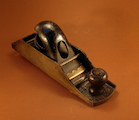
\includegraphics[height=80pt]{imagenet1.jpg}%
	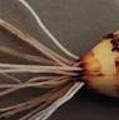
\includegraphics[height=80pt]{imagenet2.jpg}%
	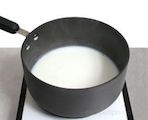
\includegraphics[height=80pt]{imagenet3.jpg}%
	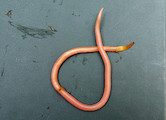
\includegraphics[height=80pt]{imagenet4.jpg}
\end{center}

这些是各自分类中的圆线刨、褐根腐菌、煮过的牛奶和常见的蛔虫。如果你正在找个挑战,
我鼓励你去访问 ImageNet 的%
\href{http://www.image-net.org/synset?wnid=n03489162}{手工具}列表,这个列表把圆
线刨、短刨、倒角刨和大概一打的其它刨子类型从其它种类中区分开。我不知道你怎么样,
但是我是没有信心区分所有这些工具的类型。这明显是一个比 MNIST 更有挑战性的图像识
别任务。LRMD 的网络获得了一个不错的 15.8\% 的准确率来正确分类 ImageNet 图像。那
听上去可能不算令人印象深刻,但是和以前的最好成绩 9.3\% 准确率相比已经是巨大的进
步了。这个跳跃暗示着神经网络也许能提供一个强大的方法来应对非常有挑战性的图像识别
任务,比如 ImageNet。\\

\textbf{2012 KSH 论文:} LRMD 的成果被一篇 Krizhevsky,
Sutskever 和 Hinton (KSH)
\footnote{\href{http://www.cs.toronto.edu/~fritz/absps/imagenet.pdf}{ImageNet
    classification with deep convolutional neural networks}, by Alex Krizhevsky,
  Ilya Sutskever, and Geoffrey E. Hinton (2012).} 的 2012 年论文追随。KSH 训练和
测试一个深度卷积神经网络,它使用 ImageNet数据的一个有限的子集。他们使用的子集来自
一个流行的机器学习竞赛 —— ImageNet Large-Scale Visual Recognition
Challenge(ILSVRC)。使用一个竞赛用的数据集给了他们一个很好的和其它领先技术比较的
途径。ILSVRC-2012 训练集包含有大约 1,200,000 幅 ImageNet 图像,取自 1,000 个种类。
验证和测试集分别包含有 50,000 和 150,000 幅图像,各自取自同样的 1,000 个种类。

运行 ILSVRC 竞赛一个困难的地方是很多 ImageNet 图像包含了多个物体。假设一幅显示一
条拉布拉多犬追逐一个足球的图像。这幅图像所谓“正确的” ImageNet 分类也许是一条拉
布拉多犬。如果一个算法把这个图像标记为一个足球,它应该被扣分吗?由于这种歧义性,
如果实际的 ImageNet 分类在一个算法认为最有可能的 $5$ 个分类中,那么这个算法就被认
为是正确的。通过这个前 $5$ 标准,KSH 的深度卷积网络达到了一个 $84.7$\% 的准确率,
大大好于次优的参赛者,后者取得了 $73.8$\% 的准确率。使用更严格的必需准确标记的标
准,KSH 的网络达到了 $63.3$\% 的准确率。

既然 KSH 网络激励了随后的成果,值得对它简要描述一下。正如我们看到的,尽管要更精细,
它非常接近于这一章中我们之前训练的网络。KSH 使用一个深度卷积神经网络,在两
个 GPU上训练。他们使用两块 GPU 是因为当时使用的特定的 GPU 型号(一块 NVIDIA
GeForce GTX 580)没有足够的片上存储器来保存整个网络。所以他们用两块 GPU 把网络分
成两个部分。

KSH 网络有 $7$ 个隐藏神经元层。前 $5$ 个隐藏层是卷积层(有些具有最大值混合),而
接下来的 $2$ 层是全连接层。输出层是一个 $1,000$ 个单元的柔性最大值层,对应于
那$1,000$ 个图像类别。这是这个网络的一个草图,取自 KSH 论文\footnote{感谢 Ilya
  Sutskever。}。细节在下面讨论。注意许多层被分成 $2$ 个部分,对应于 $2$ 块 GPU。
\begin{center}
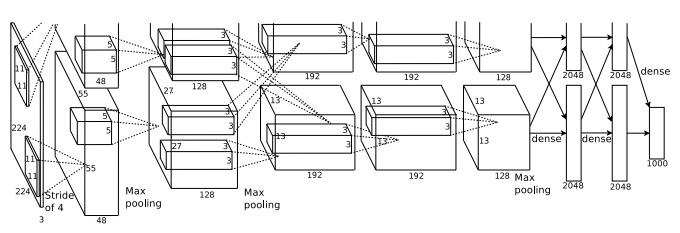
\includegraphics[width=.9\textwidth]{KSH}
\end{center}

输入层包含 $3 \times 224 \times 224$ 个神经元,对应于一幅 $224 \times 224$ 图像
的 RBG 值。回想前面提到的,ImageNet 包含有不同分辨率的图像。这引起了一个问题,因
为一个神经网络的输入层通常是固定大小。KSH 通过缩放每幅图像使得长和宽中短的长度
为 $256$ 来处理。然后他们从缩放后的图像中裁剪出一个 $256 \times 256$ 的区域。最
后,KSH 从 $256 \times 256$ 的图像中随机提取出 $224 \times 224$ 的子图像(和水平
反射)。他们把这个随机的裁剪用作扩展训练数据的方式,这样减少过度拟合。这在一个例
如 KSH 的大的网络中尤其有帮助。正是这些 $224 \times 224$ 图像被用于网络的输入。在
大多数情况下裁剪后的图像仍然包含有未改动图像的主要物体。

这是 KSH 论文中许多核心思想一个总体概况。我已经忽略了一些细节,对此你可以看下论文。
你也可以看下 Alex
Krizhevsky 的 \href{https://code.google.com/p/cuda-convnet/}{cuda-convnet}(和接
替版本),它包含有实现这许多思想的代码。一个基于 Theano 的实
现\footnote{\href{http://arxiv.org/abs/1412.2302}{Theano-based large-scale
    visual recognition with multiple GPUs}, by Weiguang Ding, Ruoyan Wang, Fei
  Mao, and Graham Taylor (2014).},代码可以
在\href{https://github.com/uoguelph-mlrg/theano_alexnet}{这里}得到。尽管使用
多 GPU 会让情况变得复杂,但代码本身还是类似于这章我们写出来的那些。Caffe 神经网络
框架也包含一个 KSH 网络的版本,详细参
见 \href{http://caffe.berkeleyvision.org/model_zoo.html}{Model Zoo}。\\

\textbf{2014 ILSVRC 竞赛:} 自 2012 年以来,研究一直在快速推进。看
看 2014 年的 ILSVRC 竞赛。和 2012 一样,这次也包括了一个 $120,000$ 张图
像,$1,000$ 种类别,而优值系数是前 $5$ 个预测是否包含正确的分类。获胜团队,主要来
自谷歌\footnote{\href{http://arxiv.org/abs/1409.4842}{Going deeper with
    convolutions}, by Christian Szegedy, Wei Liu, Yangqing Jia, Pierre Sermanet,
  Scott Reed, Dragomir Anguelov, Dumitru Erhan, Vincent Vanhoucke, and Andrew
  Rabinovich (2014).},使用了包含 $22$ 层神经元的深度卷积网络。他们称此
为 GoogLeNet,作为向 LeNet-5 的致敬。GoogLeNet 达到了 93.33\% 的前 $5$ 准确率,远
超 2013 年的获胜者(\href{http://www.clarifai.com/}{Clarifai},88.3\%)和 2012 年
的获胜者(KSH,84.7\%)。

那么 GoogLeNet 93.33\% 的准确率又是多好呢?在 2014 年,一个研究团队写了一篇关
于 ILSVRC 竞赛的综述文章\footnote{\href{http://arxiv.org/abs/1409.0575}{ImageNet
    large scale visual recognition challenge}, by Olga Russakovsky, Jia Deng,
  Hao Su, Jonathan Krause, Sanjeev Satheesh, Sean Ma, Zhiheng Huang, Andrej
  Karpathy, Aditya Khosla, Michael Bernstein, Alexander C. Berg, and Li Fei-Fei
  (2014).}。其中有个问题是人类在这个竞赛中能表现得如何。为了做这件事,他们构建了
一个系统让人类对 ILSVRC 图像进行分类。其作者之一 Andrej Karpathy 在一
篇%
\href{http://karpathy.github.io/2014/09/02/what-i-learned-from-competing-against-a-convnet-on-imagenet/}{%
  博文}中解释道,让人类达到 GoogLeNet 的性能确实很困难:

\begin{quote}
  ...the task of labeling images with 5 out of 1000 categories quickly turned
  out to be extremely challenging, even for some friends in the lab who have
  been working on ILSVRC and its classes for a while. First we thought we would
  put it up on [Amazon Mechanical Turk]. Then we thought we could recruit paid
  undergrads. Then I organized a labeling party of intense labeling effort only
  among the (expert labelers) in our lab. Then I developed a modified interface
  that used GoogLeNet predictions to prune the number of categories from 1000 to
  only about 100. It was still too hard - people kept missing categories and
  getting up to ranges of 13-15\% error rates. In the end I realized that to get
  anywhere competitively close to GoogLeNet, it was most efficient if I sat down
  and went through the painfully long training process and the subsequent
  careful annotation process myself... The labeling happened at a rate of about
  1 per minute, but this decreased over time... Some images are easily
  recognized, while some images (such as those of fine-grained breeds of dogs,
  birds, or monkeys) can require multiple minutes of concentrated effort. I
  became very good at identifying breeds of dogs... Based on the sample of
  images I worked on, the GoogLeNet classification error turned out to be
  6.8\%... My own error in the end turned out to be 5.1\%, approximately 1.7\%
  better.
\end{quote}

换言之,一个专家级别的人类,非常细心地检查图像,付出很大的努力才能够微弱胜过深度
神经网络。实际上,Karpathy 指出第二个人类专家,用小点的图像样本训练后,只能达
到 12.0\% 的 top-5 错误率,明显弱于 GoogLeNet。大概有一半的错误都是专家“难以发现
和认定正确的类别究竟是什么”。

这些都是令人惊奇的结果。确实,在这项成果后,很多团队也报告 top-5 错误率实际
上\emph{好}过 5.1\%。这有时候在媒体上被报道成系统有超过人类的视觉。尽管这些结构是
很振奋人心的,但是这样的报道只能算是一种误解,认为系统在视觉上超过了人类,事实上
并非这样。ILSVRC 竞赛问题在很多方面都是受限的 —— 在公开的网络上获得图像并不具备在
实际应用中的代表性!而且 top-5 标准也是非常人工设定的。我们在图像识别,或者更宽泛
地说,计算机视觉方面的研究,还有很长的路要走。当然看到近些年的这么多进展,还是很
鼓舞人心的。\\

\textbf{其它活动:}

\begin{center}
	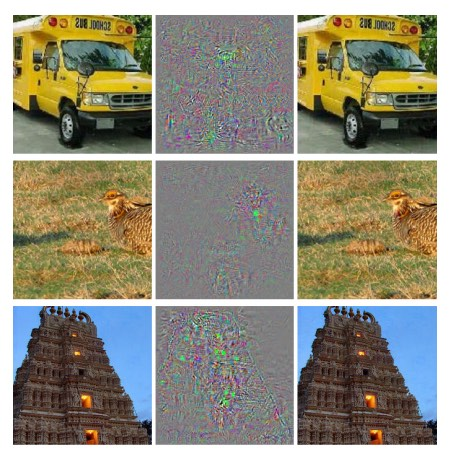
\includegraphics[width=.75\textwidth]{adversarial.jpg}
\end{center}

\section{其他的深度学习模型}
\label{sec:other_approaches_to_deep_neural_nets}

\section{神经网络的未来}
\label{sec:on_the_future_of_neural_networks}
